\documentclass{standalone}

\usepackage[english]{babel}

% to create tables, with adaptative column width
\usepackage{array}
\usepackage{tabularx}
\usepackage{adjustbox}
\usepackage{float}

% to define font size

\usepackage{ulem}
\usepackage{moresize}
\usepackage{anyfontsize}

% to use tikz and its libraries

\usepackage{tikz-timing}
\usepackage{tikz}

\usetikzlibrary{backgrounds}
\usetikzlibrary{positioning, calc, arrows,
  shapes, automata, petri, patterns}

% to use tikzmark, to place and refer to marks outside the current figure

\tikzset{every picture/.style={remember picture}}

% styles for transitions

\tikzset{transition/.append style={fill=black!20, thick}}
\tikzset{transition/.append style={fill=black!20, thick}}

% styles for test and inhib arcs.

\tikzstyle{test}=[pre, *-]
\tikzstyle{inhib}=[pre, o-]

% to use colors

\usepackage{xcolor}

%%%%%%%%%%%%%%%%%%%%%%%%%%%%%%%%%%%%%%%%%%%%%%%%%%
%                  BEGIN DOCUMENT                %
%%%%%%%%%%%%%%%%%%%%%%%%%%%%%%%%%%%%%%%%%%%%%%%%%%

\begin{document}

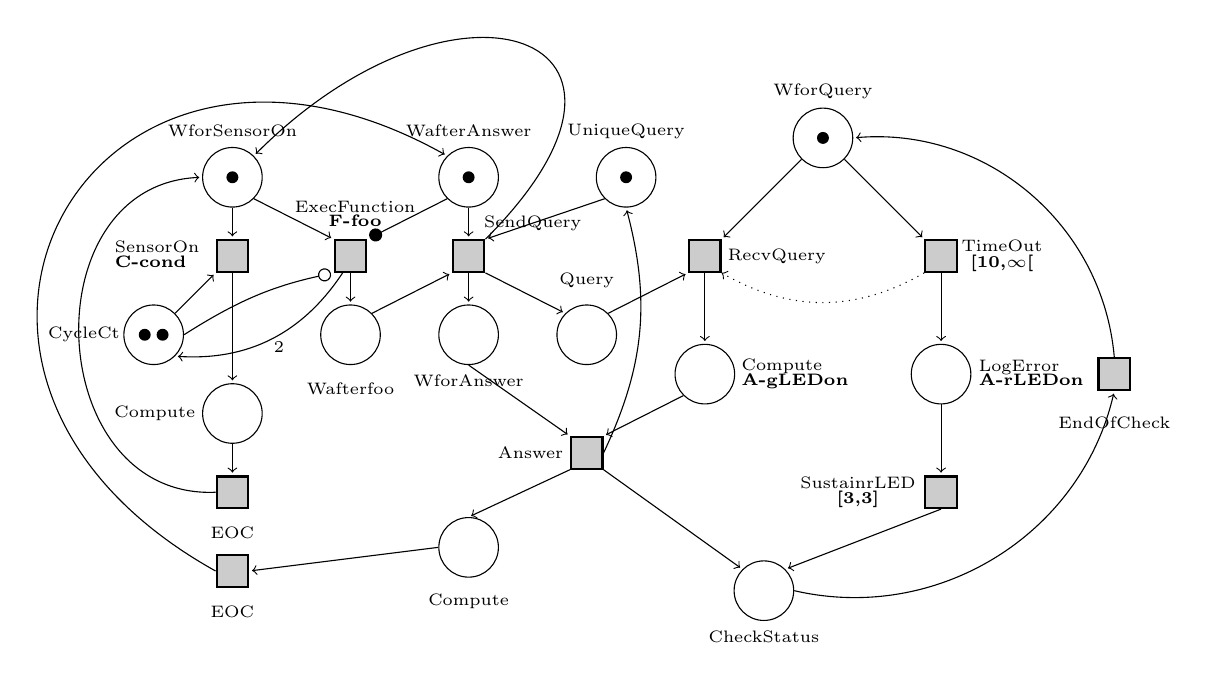
\begin{tikzpicture}
  
  %%% LEFT COMPONENT

  % \draw[help lines,step=8pt] (-2.6cm,1.9cm) grid (12cm,-6cm);
  \clip (-2.6cm,1.9cm) rectangle (12cm,-6cm); 

  % COMPONENT 1
  
  % PLACES AND TRANSITIONS
  
  \node[place,tokens=1] (wforsensoron) {};
  \node[place,tokens=1] (wafteranswer)
  at ($(wforsensoron)+(3cm,0)$) {};

  \node[transition] (sensoron) at ($(wforsensoron)-(0,1cm)$) {};
  \node[transition] (execfun)
  at ($(wforsensoron)!.5!(wafteranswer)-(0,1cm)$) {};
  \node[transition] (sendquery) at ($(wafteranswer)-(0,1cm)$) {};

  \node[place,tokens=2] (cyclect) at ($(sensoron)-(1cm,1cm)$) {};
  \node[place] (caftersensoron) at ($(sensoron)-(0,2cm)$) {};
  \node[place] (wafterfoo) at ($(execfun)-(0,1cm)$) {};
  \node[place] (wforanswer) at ($(sendquery)-(0,1cm)$) {};
  \node[place] (query) at ($(sendquery)+(1.5cm,-1cm)$) {};

  \node[transition] (eocsensoron)
  at ($(caftersensoron)-(0,1cm)$) {};
  \node[transition] (answer) at ($(query)-(0,1.5cm)$) {};
  \node[transition] (eocanswer) at ($(eocsensoron)-(0,1cm)$) {};

  \node[place] (cafteranswer) at ($(answer)-(1.5,1.2cm)$) {};

  % ARCS

  \draw
  ($(sensoron.north)$)
  edge[pre]
  ($(wforsensoron.south)$);
  
  \draw
  ($(execfun.north west)$)
  edge[pre]
  ($(wforsensoron.south east)$);

  \draw
  ($(execfun.north east)$)
  edge[test]
  ($(wafteranswer.south west)$);

  \draw
  ($(sendquery.north)$)
  edge[pre]
  ($(wafteranswer.south)$);

  \draw
  ($(execfun.south)$)
  edge[post]
  ($(wafterfoo.north)$);

  \draw
  ($(sendquery.south west)$)
  edge[pre]
  ($(wafterfoo.north east)$);

  \draw
  ($(sendquery.south)$)
  edge[post]
  ($(wforanswer.north)$);

  \draw
  ($(sendquery.south east)$)
  edge[post]
  ($(query.north west)$);

  \draw
  ($(answer.north west)$)
  edge[pre]
  ($(wforanswer.south)$);

  \draw
  ($(answer.south west)$)
  edge[post]
  ($(cafteranswer.north)$);

  \draw
  ($(sensoron.south)$)
  edge[post]
  ($(caftersensoron.north)$);

  \draw
  ($(eocsensoron.north)$)
  edge[pre]
  ($(caftersensoron.south)$);

  \draw
  ($(eocsensoron.west)$)
  edge[post,bend left=90,looseness=1.4]
  ($(wforsensoron.west)$);

  \draw
  ($(cafteranswer.west)$)
  edge[post]
  ($(eocanswer.east)$);

  \draw
  ($(sensoron.south west)$)
  edge[pre]
  ($(cyclect.north east)$);

  \draw
  ($(eocanswer.west)$)
  edge[post,bend left=90,looseness=2.2]
  ($(wafteranswer.north west)$);

  \draw
  ($(sendquery.north east)$)
  edge[post, in=45, out=45, looseness=3]
  ($(wforsensoron.north east)$);

  \draw
  ($(execfun.south west)$)
  edge[inhib,bend right=10]
  ($(cyclect.east)$);

  \draw
  ($(execfun.south)-(1mm,0)$)
  edge[post, bend left] node[xshift=1mm,yshift=-1mm]{\ssmall 2}
  ($(cyclect.south east)$);

  % LABELS

  \node (lwforsensoron)
  at ($(wforsensoron.north)+(0,2mm)$) {\ssmall WforSensorOn};

  \node (lwafteranswer)
  at ($(wafteranswer.north)+(0,2mm)$) {\ssmall WafterAnswer};

  \node (lwafteranswer)
  at ($(sensoron.west)-(8mm,0)$) {
    \renewcommand\arraystretch{.3}
    \begin{tabular}{@{}l@{}}
      \ssmall SensorOn \\
      {\ssmall\bf C-cond} \\
    \end{tabular}

  };

  \node (lexecfun)
  at ($(execfun.north)+(0,3mm)$) {
    \renewcommand\arraystretch{.3}
    \begin{tabular}{@{}c@{}}
      \ssmall ExecFunction \\
      {\ssmall\bf F-foo} \\
    \end{tabular}

  };

  \node (lcyclect)
  at ($(cyclect.west)-(5mm,0)$) {\ssmall CycleCt};

  \node (lwafterfoo)
  at ($(wafterfoo.south)-(0,3mm)$) {\ssmall Wafterfoo};

  \node (lsendquery)
  at ($(sendquery.north east)+(6mm,2mm)$) {\ssmall SendQuery};

  \node (lwforanswer)
  at ($(wforanswer.south)-(0,2mm)$) {\ssmall WforAnswer};

  \node (lquery)
  at ($(query.north)+(0,3mm)$) {\ssmall Query};

  \node (lanswer)
  at ($(answer.west)-(5mm,0)$) {\ssmall Answer};

  \node (lcaftersensoron)
  at ($(caftersensoron.west)-(6mm,0)$) {\ssmall Compute};

  \node (leocsensoron) 
  at ($(eocsensoron.south)-(0,3mm)$) {\ssmall EOC};

  \node (leocanswer) 
  at ($(eocanswer.south)-(0,3mm)$) {\ssmall EOC};

  \node (lcafteranswer) 
  at ($(cafteranswer.south)-(0,3mm)$) {\ssmall Compute};  

  % COMPONENT 2
  
  % PLACES AND TRANSITIONS

  \node[place, tokens=1] (uniqquery)
  at ($(query)+(.5cm,2cm)$) {};
  
  \node[place, tokens=1] (wforquery) at ($(uniqquery)+(2.5,.5cm)$) {};

  \node[transition] (recvquery) at ($(wforquery)-(1.5cm,1.5cm)$) {};
  \node[transition] (timeout) at ($(wforquery)+(1.5cm,-1.5cm)$) {};

  \node[place] (computeans) at ($(recvquery)-(0,1.5cm)$) {};
  \node[place] (logerr) at ($(timeout)-(0,1.5cm)$) {};

  \node[transition] (endofcheck) at ($(logerr)+(2.2cm,0)$) {};
  \node[transition] (sustainrled) at ($(logerr)-(0,1.5cm)$) {};

  \node[place] (checkstatus)
  at ($(answer)!.5!(sustainrled)-(0,1.5cm)$) {};

  % ARCS

  \draw
  ($(timeout.south west)$)
  edge[dotted,->,bend left]
  ($(recvquery.south east)$);
  
  \draw
  ($(recvquery.south west)$)
  edge[pre]
  ($(query.north east)$);

  \draw
  ($(sendquery.north east)$)
  edge[pre]
  ($(uniqquery.south west)$);
  
  \draw
  ($(recvquery.north east)$)
  edge[pre]
  ($(wforquery.south west)$);

  \draw
  ($(timeout.north west)$)
  edge[pre]
  ($(wforquery.south east)$);

  \draw
  ($(recvquery.south)$)
  edge[post]
  ($(computeans.north)$);

  \draw
  ($(timeout.south)$)
  edge[post]
  ($(logerr.north)$);

  \draw
  ($(answer.north east)$)
  edge[pre]
  ($(computeans.south west)$);
  
  \draw
  ($(sustainrled.north)$)
  edge[pre]
  ($(logerr.south)$);

  \draw
  ($(answer.south east)$)
  edge[post]
  ($(checkstatus.north west)$);

  \draw
  ($(sustainrled.south)$)
  edge[post]
  ($(checkstatus.north east)$);

  \draw
  ($(answer.east)$)
  edge[post, bend right=20]
  ($(uniqquery.south)$);

  \draw
  ($(endofcheck.south)$)
  edge[pre,bend left=45]
  ($(checkstatus.east)$);

  \draw
  ($(endofcheck.north)$)
  edge[post,bend right=45]
  ($(wforquery.east)$);

  % LABELS

  \node (lwforquery)
  at ($(wforquery.north)+(0,2mm)$) {\ssmall WforQuery};

  \node (luniqquery)
  at ($(uniqquery.north)+(0,2mm)$) {\ssmall UniqueQuery};

  \node (lrecvquery)
  at ($(recvquery.east)+(7mm,0)$) {\ssmall RecvQuery};

  \node (ltimeout)
  at ($(timeout.east)+(5mm,0)$) {
    \renewcommand\arraystretch{.3}
    \begin{tabular}{@{}c@{}}
      \ssmall TimeOut \\
      {\ssmall\bf [10,$\infty$[} \\
    \end{tabular}        
  };

  \node (lcomputeans)
  at ($(computeans.east)+(7mm,0)$) {
    \renewcommand\arraystretch{.3}
    \begin{tabular}{@{}l@{}}
      \ssmall Compute \\
      {\ssmall\bf A-gLEDon} \\
    \end{tabular}        
  };

  \node (llogerr)
  at ($(logerr.east)+(7mm,0)$) {
    \renewcommand\arraystretch{.3}
    \begin{tabular}{@{}l@{}}
      \ssmall LogError \\
      {\ssmall\bf A-rLEDon} \\
    \end{tabular}        
  };

  \node (lcheckstatus)
  at ($(checkstatus.south)+(0,-2mm)$) {\ssmall CheckStatus};

  \node (lsustainrled)
  at ($(sustainrled.west)+(-9mm,0)$) {
    \renewcommand\arraystretch{.3}
    \begin{tabular}{@{}c@{}}
      \ssmall SustainrLED \\
      {\ssmall\bf [3,3]} \\
    \end{tabular}        
  };

  \node (lendofcheck)
  at ($(endofcheck.south)+(0,-4mm)$) {\ssmall EndOfCheck};
    
\end{tikzpicture}

\end{document}

%%% Local Variables:
%%% mode: latex
%%% TeX-master: t
%%% End:
